% Träddiagram av polymertyperna:
%Ref: PolyT p. 5
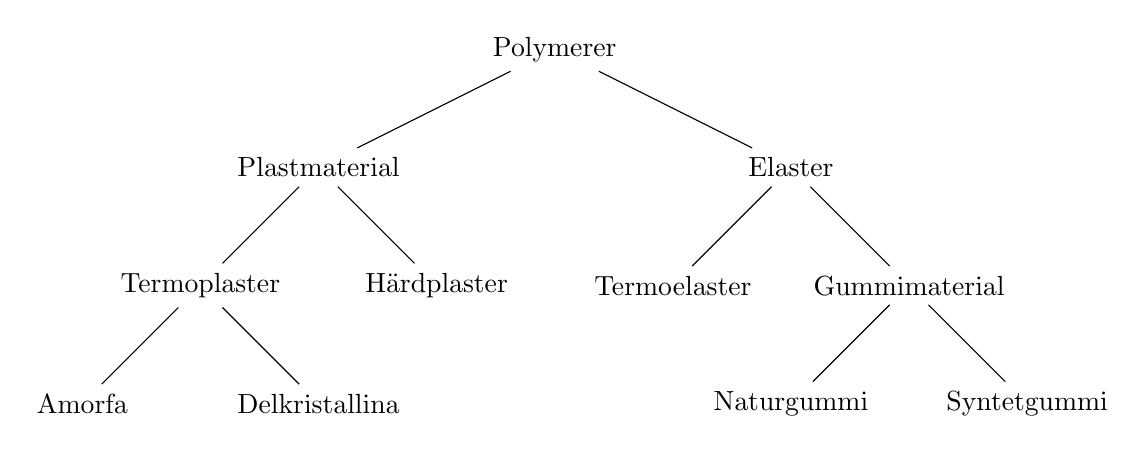
\begin{tikzpicture}[
    level 1/.style={sibling distance=6cm},
    level 2/.style={sibling distance=3cm},
    level 3/.style={sibling distance=3cm}
  ]
    \node {Polymerer}
        child { node {Plastmaterial}
            child { node {Termoplaster} 
                child { node {Amorfa} }
                child { node {Delkristallina} }    
            }
            child { node {Härdplaster} }
        }
        child { node {Elaster}
            child { node {Termoelaster} }
            child { node {Gummimaterial} 
                child { node {Naturgummi} }
                child { node {Syntetgummi} }
            }
        };
\end{tikzpicture}
